
\newcommand{\argmaxs}[2]{\arg \max_{#2}{#1}}

\chapter{Exercises}

\section{Bayes}

\subsection{Naive Bayes Classifier}

\begin{figure}[H]
    \centering
   \includegraphics[scale=0.5]{exercises/bayes/ex1.png}
\end{figure}


\paragraph{Naive description and difference}
So the optimal one is equal to:
$$c_{ob}=P(c_j|x,D)=\sum_h P(c_j|x,h)P(h|D)$$
Which requires to estimate all the hypos probabilities.\\
So this is where the naive classifiers comes into pay saying that the sample $x$ can be seen as a set of attributes $A=\{a_1,a_2,\dots, a_n\}$ which are \textbf{independent} from each other.\\
It does so using the  bayes theorem in the following way:
$$P(c_j|x,D)=P(c_j|A,D)=\frac{P(A|c_j,D)P(c_j|D)}{P(A|D)}=P(A|c_j,D)P(c_j|D)=P(c_j|D)\prod_i P(a_i|c_j,D)$$
So now the classifiers becomes
$$C_{NB}=\argmax_{c_i \in C}P(c_j|D)\prod_i P(a_i|c_j,D)$$
Since the $P(x| c_i,D)$ factor can be difficult to compute when there are many attributes of $x$, the naive bayes classifier assumes that each attribute is independent, so that.

\paragraph{Implementation }
In Multinomial Naïve Bayes each $p(c)$ is a multinomial distribution, so it is possible to solve the classification problem of documents using Multinomial Naïve Bayes because multinomial distribution works well for data which can easily be turned into counts, such as word counts in a text.
Given:
\begin{itemize}
\item $P(c_j)$: probability of class $c_j$
\item $P(w_i|c_j)$: probability of the word $w_i$ given the class $c_j$.
\end{itemize}
We must estimate $P(c_j)$ and $P(w_i|c_j)$ using multinomial distribution, then use them to classify a new document. Remove every word in the documents not appearing in the vocabulary V build in the previous phase and then use:
\[V_{NB}=\argmaxs{P(c_j)\prod_{i=1}^{lenght(d)}P(w_i|c_j,D)}{c_j \in C}\]


\subsection{MAP, ML, optimality}
\begin{figure}[H]
    \centering
   \includegraphics[scale=0.5]{exercises/bayes/ex2.png}
\end{figure}

\paragraph{Define MAP and ML }
Both the MAP and ML try to get the hypo which maximize the probability $p(h|D)$ in following way:

$$MAP=\argmax_{h \in H} p(h|D)=\argmax_{h \in H} p(D|h)p(h)$$

When the prior for every hypo is the same then we can drop the $p(h)$ factor:

$$ML=\argmax_{h \in H} p(h|D)=\argmax_{h \in H} p(D|h)$$

\paragraph{Bayes optimal classifier}
Since the previous do not take into account the classification given by multiple hypos we use an optimal classifier as:
$$C_{B}=\argmax_{c_i \in C}\sum_{h_j \in H} p(c_i| h_j,x)p(h_j|D)$$
That is we get the class which yields the higher sum of two elements: the probability that the element $x$ is classified as $c_i$ by $h_j$ and the probability that $h_j$ in $D$.

\paragraph{Practical use}
The applicability should be for simple tasks such as predicting the gender of a dataset consisting of heights and weights.


\subsection{ML}
\begin{figure}[H]
    \centering
   \includegraphics[scale=0.5]{exercises/bayes/ex3.png}
\end{figure}

\paragraph{Definition}
ML is derived using the bayes theorem when the prior for each hypo is the same $p(h_1)=p(h_2)=...=p(h_n)$.
The ML returns the hypo which maximizes $p(h|D)$ as follows:
$$ML=\argmax_{h_i \in H}p(D|h)$$

\paragraph{Comment}
The ML returns the most probable hypo which then may or may not correctly classify the element.

\subsection{Exercise}
\begin{figure}[H]
    \centering
    \includegraphics[scale=0.5]{exercises/bayes/ex4.png}
\end{figure}

\paragraph{point 1}
We want to estimate $p(C_1|x)$. Using the bayes rules we have:
$$p(C_1|x)=p(x|C_1)P(C_1)$$
Where $p(x|C_1)=N(x;\mu_1, \Sigma)$

\paragraph{Express in terms of sigma}
To solve this let's start from $\sigma(\alpha)$ and work out way back to $P(C_1|x)$. First let's use:
$$\tau=\frac{P(x|C_1)P(C_1)}{P(x|C_2)P(C_2)}$$
So we can write
$$\sigma(\alpha)=\frac{1}{1+e^{-\alpha}}=\frac{e^{\alpha}}{1+e^{\alpha}}=\frac{\tau}{1+\tau}$$
Let's focus on the denominator:
$$\tau+1=\frac{P(x|C_1)P(C_1)}{P(x|C_2)P(C_2)}+1=\frac{P(x|C_1)P(C_1)+P(x|C_2)P(C_2)}{P(x|C_2)P(C_2)}=\frac{1}{P(x|C_2)P(C_2)}$$
So we get:
$$\frac{\tau}{1+\tau}=\frac{P(x|C_1)P(C_1)}{P(x|C_2)P(C_2)}\cdot P(x|C_2)P(C_2)=P(x|C_1)P(C_1)$$
So we can say that:
$$P(C_1|x)=P(x|C_1)P(C_1)=\sigma(\alpha)$$

\paragraph{Model Parameters}
The model parameters are defined by $N(x;\mu_1, \Sigma)$, so we have 2 means ($\mu_1,\mu_2$) and 4 others since $\Sigma$ has dimension $2 \times 2$ and it's the same for both classes. So we get a total of 6 parameters.

\section{MDP, RL}
\subsection{Definitions}

\begin{figure}[H]
    \centering
     \includegraphics[scale=0.5]{exercises/mdp/ex1.png}
\end{figure}

\paragraph{Markov properties} once the current state is known, the evolution of the dynamic system does not depend on the history of states, actions and observations. The current state contains all the information needed to predict the future. Future states are conditionally independent of past states and past observations given the current state. The knowledge about the current state makes past, present and future observations statistically independent. Markov process has Markov properties.\\


\paragraph{MDP}
\begin{figure}[H]
    \centering
    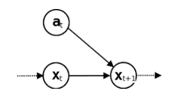
\includegraphics[scale=1]{MDP.png}
\end{figure}

An MDP is for decision making where the states are fully observable, hence there is  no need of observations. In presence of non-deterministic or stochastic actions, they can be fully observed after its execution.\\
Having 
\begin{itemize}
\item $X$ finite set of states:
\item $A$: finite set of actions
\item Deterministic $\delta: X\times A \rightarrow X$: a function which maps an action-state tuple to the next state.
\item Non-deterministic $\delta: X\times A \rightarrow 2^X$.
\item Stochastic $\delta: P(x'|x,a)$: the probability of having he state $x'$ given previous state $x$ and action $a$.
\item Deterministic $r:X\times A \rightarrow R$: a function which maps a tuple state-action to a reward.
\item Non-deterministic/Stochastic $r:X\times A \times X \rightarrow R$
\end{itemize}
An MDP is made of $MSP=\braces{X,A,\delta,r}$

\paragraph{HMM}
\begin{figure}[H]
    \centering
    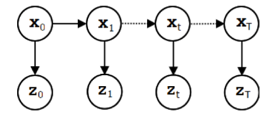
\includegraphics[scale=1]{HMM.png}
\end{figure}

In a HMM sate states $x_t$ are discrete and not observable, while the observations $z_t$ can be either discrete or continuous. Finally there is no control over the system.\\
Given:
\begin{itemize}
\item $X$: set of not observable states
\item $Z$: set of observations
\item $P(x_t|x_{t-1})$: the transition model 
\item $P(z_t|x_t)$: an observation models which maps the probability of having an observation $z_t$ to a state $x_t$.
\item $\pi_0$: an initial distribution
\item $\bm{A}=\braces{A_{ij}}=P(x_t=j|x_{t-1}=i)$ a transition matrix
\item $b_k(z_t)=P(z_t|x_t=k)$ an observation model.
\item $\pi_0=P(x_0)$: an initial probability.
\end{itemize}
We have that a HMM is made of $HMM=\braces{X,Z,\pi_0}$.

\subsection{Exercise}

\begin{figure}[H]
    \centering
    \includegraphics[scale=0.8]{exercises/mdp/ex2.png}
\end{figure}

\paragraph{Complete model}
An MDP has the four components:
\begin{itemize}
\item Set of states $X=\{x_1,x_2\}$: Since the action is crossing the bridge, the states indicate on which part of the bridge the car currently is.
\item Set of actions $A=\{b_1,b_2,b_3\}$: contains the three possible bridges to choose.
\item A deterministic transition function $\gamma$: which is independent of the action since the car will always cross the bridge to get to the other side
\item A reward function $r: X\times A$, which takes as input a state and an action and returns the time. 
\end{itemize}


\subsection{Exercise}

\begin{figure}[H]
    \centering
    \includegraphics[scale=0.5]{exercises/mdp/ex3.png}
\end{figure}

\paragraph{Definition}
A RL problem includes an agent accomplishing a task according to an  MDP $(X, A, \gamma, r )$, for which functions $\gamma$ and $r$ are unknown to the agent. The aim is to find an optimal policy $\pi$ which maximizes the a value function $V$ 

\paragraph{Main Steps}
Givan an MDP the agent start executing random actions and saves the triple (state, action, reward) on a table. As the training continues the agent is able to map the current state to a saved triple, thus choosing the action which maximizes the reward.\\

\subsection{K-armed bandit}

\begin{figure}[H]
    \centering
    \includegraphics[scale=0.5]{exercises/mdp/ex4.png}
\end{figure}

\paragraph{Description}
The k-armed bandit problem is a problem highlighting the tradeoff between exploration and exploitation.\\
There are K slot machines each one with a probability distribution, and the goal is for a player to maximize the total reward.

\paragraph{Optimal policy}
An optimal policy is given by the Upper-Confidence-Bound:
$$A=\argmax_a[Q_t(a)+c\sqrt{\frac{2ln(t)}{N_t(a)}}]$$
Where:
\begin{itemize}
\item $Q_t(a)$ is the reward associated with pulling the arm $a$, which can also been simply the mean reward given by $a$.
\item $c$: coefficient to control tradeoff
\item $t$: current iteration
\item $N_t(a)$: times arm $a$ was pulled
\end{itemize}





\section{Linear Regression, Classification}

\subsection{Sequential vs Batch }

\begin{figure}[H]
    \centering
    \includegraphics[scale=0.8]{exercises/linear/regression/ex1.png}
\end{figure}
 

\paragraph{Linear regression}
The goal of regression is to predict the value of one or more continuous target variables $Y=\mathcal{R}$ given the value of a D-dimensional vector of input variables $X \subset \mathcal{R}^D$. The simplest linear model for regression is one that involves a linear combination of the input variables:
\[y(x,w)=w_0+w_1x_1+...+w_Dx_D=\bm{w^Tx}\]
Where $x_0=1$.

\paragraph{Batch vs sequential}


We have that a target value is given by:
\[t=y(x,w) + \epsilon\]
Where $\epsilon$ is some Gaussian noise. If we assume the samples to be i.i.d. then we can use the maximum likelihood and have:
\[max[P(\braces{t_1,...,t_n}|x_1,...,x_n,w,\beta)]\]
where $\beta^{-1}$ is the variance of the noise. This approach is used with batch learning in which the entire training set is processed altogether.\\

For sequential learning \textit{stochastic gradient descent} can be used to update the model parameters in the following way:
\[w_{n+1}=w_n+\eta \nabla E_n= w_n +[t_n -w_n^T \phi(x_n)]\phi(x_n)\]
Where:
\begin{itemize}
\item $\eta$: is the learning rate 
\item $\phi(x_n)$ : is a non linear transformation of the input vector
\end{itemize}

\subsection{Logistic Regression }

\begin{figure}[H]
    \centering
    \includegraphics[scale=0.6]{exercises/linear/regression/ex2.png}
\end{figure}
 
 \paragraph{Definition}
The Logistic regression is a classification method based on maximum likelihood.
The likelihood function is given by:
$$p(t|w)=\prod_n y_n^{t_n}(1-y_n)^{1-t_n}$$
Where $y_n$ is the predicted class for the n element, that is $\sigma(w^tx_n)$. The prediction is estimated using the non linearity $\sigma(w^tx_n)$.

\paragraph{Parameters}
The parameters to be learn are just 3, 2 for the attributes + the bias term.

\paragraph{Error Function}
The cross-entropy error function of the kind:
$$E(w)=-ln(p(t|w))$$

\subsection{Exercise }

\begin{figure}[H]
    \centering
    \includegraphics[scale=0.5]{exercises/linear/regression/ex3.png}
\end{figure}

\paragraph{Description}
To perform such regression a linear model with a polynomial curve fitting can be used of the form:
$$y=\sum_i w_ix^i$$
In such case the model should have $i \ge 3$, that is $W=w_0,w_1,w_2,w_3$.\\
The training algorithm can be a simple SDG.

\paragraph{Overfitting}
To reduce overfitting a regularization term can be introduced during the model updates .


\subsection{Classification}


\begin{figure}[H]
    \centering
    \includegraphics[scale=0.7]{exercises/linear/classification/ex1.png}
\end{figure}

The goal in classification is to take an input vector $x$ and to assign it to one of $K$  discrete classes $C_k$ where $k=1,...,K$. In the most common scenario, the classes are taken to be disjoint, so that each input is assigned to one and only one class. Data sets whose classes can be separated exactly by linear decision surfaces are said to be linearly separable. There are various ways of using target values to represent class labels.\\
For probabilistic models, the most convenient, in the case of two-class problems, is the binary representation in which there is a single target variable $t \in \braces{0,1}$ such that $t=1$ represents class $C_1$  and $t=0$  represents class $C_2$. The value of $t$ can be viewed as representing the probability of belonging to the class $C_1$.\\
For $K>2$  it is convenient to use a 1-of-K coding scheme, which is a vector $T=\braces{t_1,t_2,...,t_n}$ of length $K$ such that if the class is $C_j$, for some sample $x_i \in X,\ |X|=n$ , then the value of $t_i$ is zero everywhere except for $t_i^j$ which is one. \\
Given a dataset in the form $D=\braces{(x_n,t_n)^N_{n=1}}$ we want to find a linear discriminant $y(x)=W^Tx$, hence we minimize the sum of squares error function:
\[E(W)=\frac{1}{2}Tr\braces{(XW-T)^T(XW-T)}\]
obtaining:
\[W=(X^TX)^{-1}X^TT\]
\[y(x)=W^Tx\]
Unfortunately, least squares solutions lack robustness to outliers and are highly sensitive to them, unlike logistic regression.

\begin{figure}[H]
    \centering
    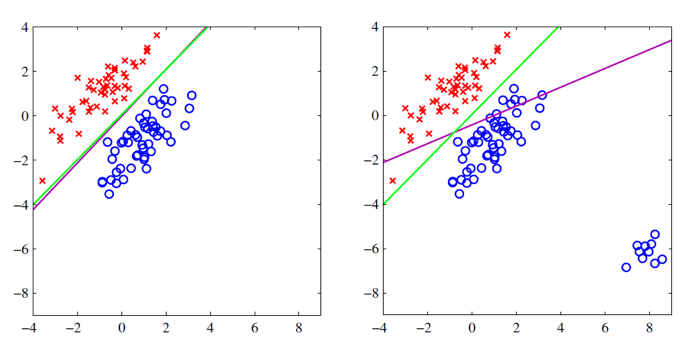
\includegraphics[scale=0.4]{least_square_error.png}
\end{figure}
The left plot shows data from two classes (red crosses and blue circles) with the decision boundary found by least squares (magenta) and by the logistic regression model (green). The right plot shows the corresponding results obtained when extra data points (outliers) are added at the bottom left of the diagram.

\section{K-NN}

\subsection{Algo and example}

\begin{figure}[H]
    \centering
    \includegraphics[scale=0.8]{exercises/k/ex1.png}
\end{figure}

\paragraph{Main steps}
Classification with K-NN, having a target function $f:X\rightarrow C$ and a dataset $D=\braces{(x_i,y_i)^N_{i=1}}$ is :
\begin{itemize}
\item Find K nearest neighbors of the new instance $x'$
\item assign $x'$ to the most common label among the majority of the neighbors.
\end{itemize}
We can estimate the likelihood of $x'$ belonging to the class $c$ as:
$$p(c| x',D,K)=\frac{1}{K}\sum_{i \in N_k(x',D)}\mathcal{I}(y_i=c)$$
with:
\begin{itemize}
\item $ N_k(x',D)$ is the set of K nearest points to $x'$
\item $\mathcal{I}(y_i=c)$ is one if the label $y_i$ is equal to $c$, zero otherwise
\end{itemize}


\begin{figure}[H]
    \centering
    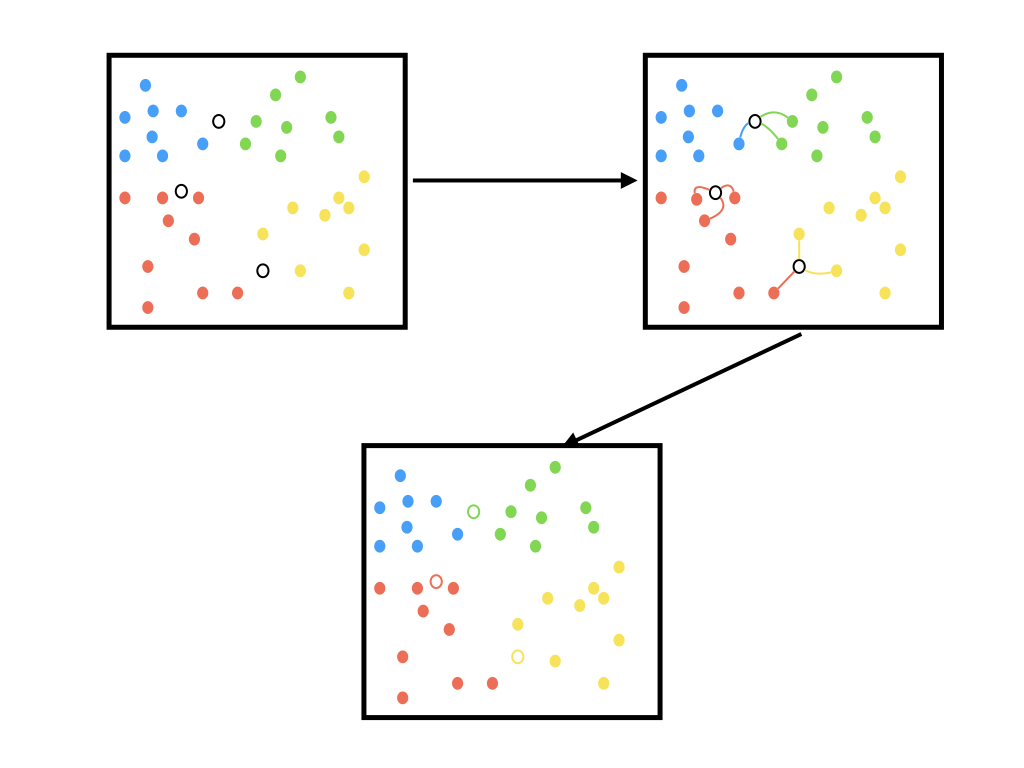
\includegraphics[scale=0.3]{knn.jpeg}
\end{figure}




\subsection{Algo and exercise}
    \begin{figure}[H]
     \centering
    \includegraphics[scale=0.5]{exercises/k/ex2.png}
\end{figure}

\paragraph{Description}
The K-NN algorithm is used in classification problems as follows:
\begin{itemize}
\item Set a number of neighbors K
\item Select an element $x$ and count the closer $k$ neighbors.
\item set $x$ to be the most common class among the neighbors.
\end{itemize}

\paragraph{Exercise}
Again, you just need to check which points are closer to the circle. 
\begin{itemize}
\item K=1 : the square is the closer, since we count just the first neighbors we can set the class to be a square.
\item K=3: the closer 3 elements are 2 triangles and 1 square, so the class is triangle.
\item K=5: just count, 3 squares and 2 triangles, so square.
\end{itemize}





\section{Tree}

\subsection{Tree classification}
\begin{figure}[H]
    \centering
    \includegraphics[scale=0.7]{exercises/tree/ex1.png}
\end{figure}

\paragraph{Rules}
\begin{enumerate}

\item $c_1 \wedge b_1 \Rightarrow No $
\item $c_1 \wedge b_2 \Rightarrow Yes $
\item $c_2 \wedge a_1 \Rightarrow Yes $
\item $c_2 \wedge a_2 \wedge b_1 \Rightarrow Yes $
\item $c_2 \wedge a_2 \wedge b_2 \Rightarrow No $
\item $c_2 \wedge a_3 \Rightarrow No $
\item $c_3  \Rightarrow No $
\end{enumerate}

\paragraph{Consistency}
\begin{itemize}
\item $s_1$ is consistent because of  1 
\item $s_2$ is consistent because of  4
\item $s_3$ is not consistent because of  7 
\item $s_4$ is not consistent because of  5
\end{itemize}

\subsection{Tree overfitting}
\begin{figure}[H]
    \centering
    \includegraphics[scale=0.8]{exercises/tree/ex2.png}
\end{figure}

\paragraph{Definition}
The definition of overfitting is the production of an analysis that corresponds too closely or exactly to a particular set of data, and may therefore fail to fit additional data or predict future observations reliably

\paragraph{Overfitting in Trees}
To avoid overfitting we can stop growing the tree when data split  are not statistically significant  or grow a full tree, then post-prune

\subsection{Tree exercise}
\begin{figure}[H]
    \centering
    \includegraphics[scale=0.5]{exercises/tree/ex3.png}
\end{figure}

\paragraph{Formalization}
The dataset consists of  5 samples each having 3 attributes.\\
2 attributes are boolean while the last one (number of rooms) is categorical, even tho there are only two possible alternatives so it can be considered boolean too.\\
The target function is of the kind $f:B^3 \to B$ where $B=\{0,1\}$.

\paragraph{Attributes}
The best attribute is decided trough the minimization of entropy, that is the attribute with the max info gain is chosen.


\paragraph{Simulation short}
\begin{figure}[H]
    \centering
    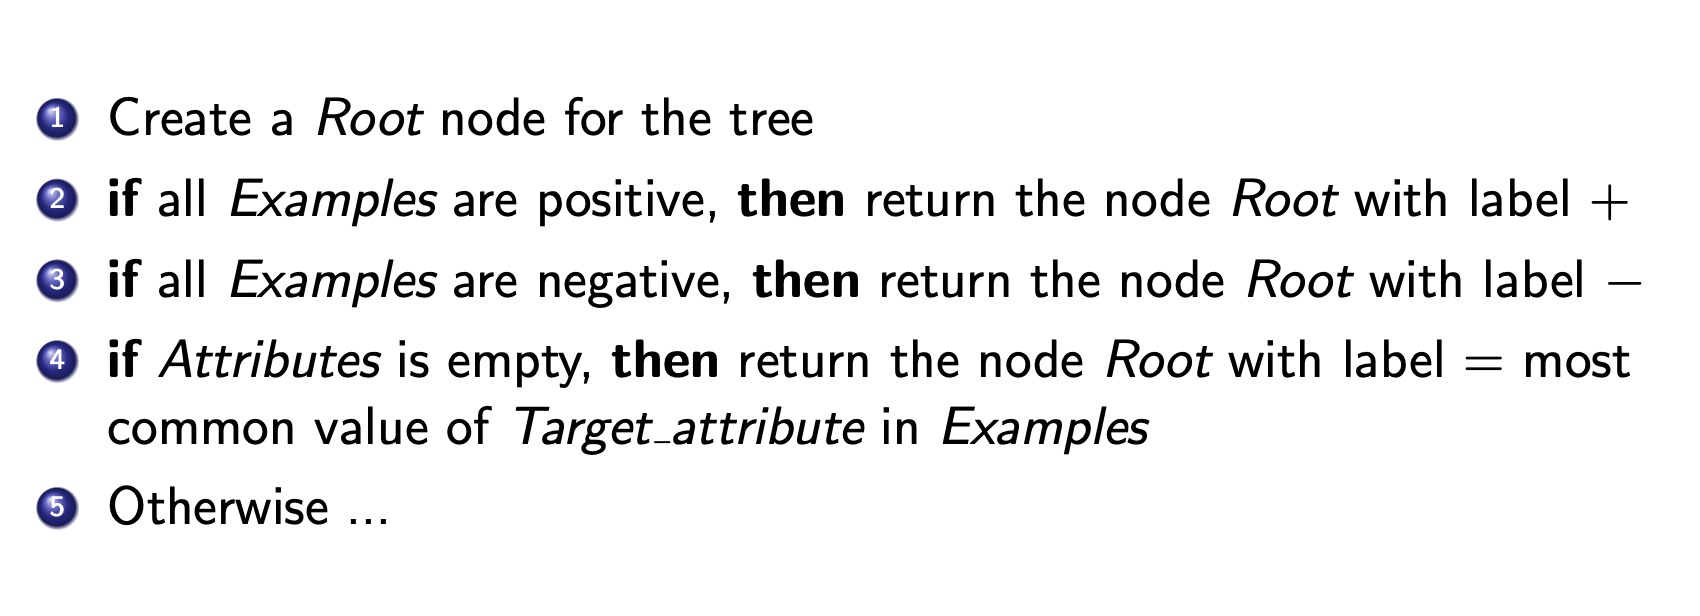
\includegraphics[scale=0.5]{exercises/tree/ex3algo.png}
\end{figure}


By observing the ID3 algorithm and the data you can easily tell how the tree is supposed to be.\\
By using rules 2,3,4 you can assest that:
\begin{itemize}
\item When there are 4 rooms the answer is always yes. So nr rooms should be the root of the node since it can discern between positive and negative.
\item When there are 3 rooms having a kitchen or not is proportional to the house being acceptable. So we can use this feature as the next node and we are done since we described all the possible outcomes. 
\end{itemize}

\paragraph{Simulation long}
Here we do not apply the immediate rules and use the minimization of entropy.\\

First we need to select the root node using the minimization of the entropy.\\
There are a total of 3 positive and 2 negative in the acceptable col, so $S=[3+,2-]$.\\
We first estimate the total entropy as:
$$Ent(S)=-p_+log_2p_+ -p_- log_2p_-=-\frac{2}{5}log_2\frac{2}{5}-\frac{3}{5}log_2\frac{3}{5}=0.97095059$$
Then we estimate the info gain for each attribute as:
$$Gain(S,A)=Ent(S)-\sum_{v \in Values(A)}\frac{|S_v|}{|S|}Ent(S_v)$$
For the furniture attribute we have :
\begin{itemize}
\item $S_+=[1+,1-]$: for each positive value of furniture how many positive/negative acceptable?
\item $S_-=[2+,1-]$: for each negative value of furniture how many positive/negative acceptable?
\end{itemize}
So now we can focus no the second term:
\begin{equation}
\begin{aligned}
-\sum_{v \in Values(Fur)}\frac{|S_v|}{|S|}Ent(S_v)=-\frac{|S_+|}{|S|}Ent(S_+)-\frac{|S_-|}{|S|}Ent(S_-)= \\
-\frac{2}{5}(-\frac{1}{2}\cdot log_2\frac{1}{2}-\frac{1}{2}\cdot log_2\frac{1}{2})-\frac{3}{5}(-\frac{2}{3}\cdot log_2\frac{2}{3}-\frac{1}{3}\cdot log_2\frac{1}{3})=\\
-\frac{2}{5}\cdot 0.928 - -\frac{3}{5}\cdot 0.993=-0.967
\end{aligned}
\end{equation}

So the furniture gain is $Gain(S,Furniture)=Ent(S)-0.967=0.039$\\

Same thing can be done with nRooms:
\begin{itemize}
\item $S_3=[1+,2-]$.
\item $S_4=[2+,0-]$. 
\end{itemize}
$Gain(S,nRoom)=0.0234$
And newKitchen:
\begin{itemize}
\item $S_+=[2+,0-]$.
\item $S_-=[1+,2-]$. 
\end{itemize}
$Gain(S,newKitchen)=0.0124$

The gain values are made up since It took to much time to to id properly, but the formulas are correct.\\

So we choose the attribute with the most info gain as our root one, Furniture. For the next attributes you just keep doing the same procedures until you come up with. From the online tool the tree is like this:

\begin{figure}[H]
    \centering
    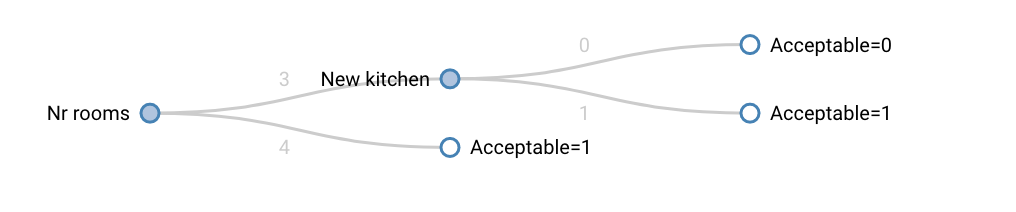
\includegraphics[scale=0.6]{exercises/tree/ex3tree.png}
\end{figure}

\section{Definitions}

\subsection{Unsupervised vs supervised}
\begin{figure}[H]
    \centering
    \includegraphics[scale=0.75]{exercises/definitions/ex1.png}
\end{figure}

Supervised learning is typically done in the context of:
\begin{itemize}
\item \textbf{Classification}: when we want to map input to output labels.
\item \textbf{Regression}: when we want to map input to a continuous output.
\end{itemize} 

In both regression and classification, the goal is to find specific relationships or structure in the input data that allow us to effectively produce correct output data.\\

Unsupervised learning uses techniques such as clustering, representation learning and density estimation. In all of these cases, we wish to learn the inherent structure of our input data without using explicitly-provided labels. Since no labels are provided, when analyzing the output there is no specific way to compare model performance in most unsupervised learning methods.\\
 
On the other hand, supervised learning  intends to infer a conditional probability distribution $p_X(x|y)$ conditioned on the label $y$ of input data; unsupervised learning intends to infer an a priori probability distribution $P_X(x)$ . Compared to supervised learning where training data is labeled with the appropriate classifications, models using unsupervised learning must learn relationships between elements in a data set and classify the raw data without "help."

\subsection{Unsupervised}
\begin{figure}[H]
    \centering
    \includegraphics[scale=0.8]{exercises/definitions/ex2.png}
\end{figure}

\paragraph{Definition}
Unsupervised learning is a branch of machine learning that learns from test data that has not been labeled, classified or categorized. Instead of responding to feedback, unsupervised learning identifies commonalities in the data and reacts based on the presence or absence of such commonalities in each new piece of data. Alternatives include supervised learning and reinforcement learning. 

\paragraph{Example}
Using K-Means with number of clusters equal to 4, we get 

\begin{figure}[H]
    \centering
    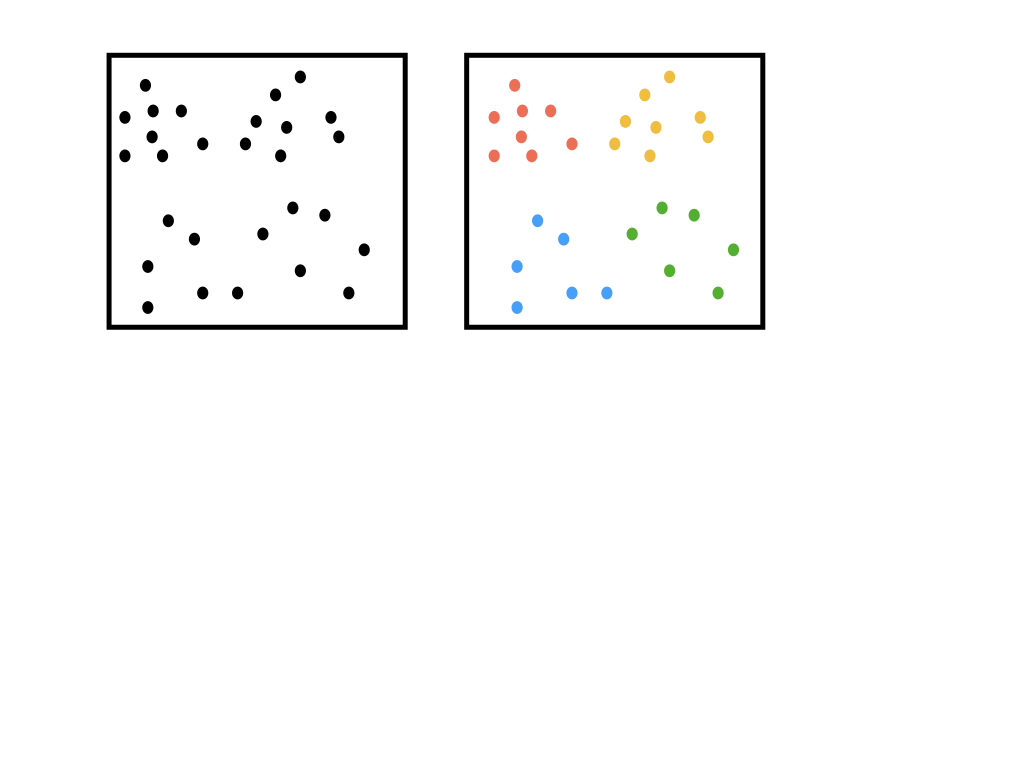
\includegraphics[scale=0.4]{kmeans.jpeg}
\end{figure}

\paragraph{K-Means}
Steps for k-means:
\begin{enumerate}
\item Set k
\item partition data randomly and define centroids
\item For each sample estimate its distance from the current centroid. If the distance is more than another centroid switch.
\item repeat previous step until convergence
\end{enumerate}


\subsection{Confusion matrix }


\begin{figure}[H]
    \centering
    \includegraphics[scale=0.5]{exercises/definitions/ex3.png}
\end{figure}

\paragraph{Definition}
A confusion matrix is a table layout that allows visualization of the performance of an algorithm.  Each row of the matrix represents the instances in a predicted class while each column represents the instances in an actual class (or vice versa).

\paragraph{Example}

% Please add the following required packages to your document preamble:
% \usepackage[table,xcdraw]{xcolor}
% If you use beamer only pass "xcolor=table" option, i.e. \documentclass[xcolor=table]{beamer}
\begin{table}[H]
\centering
\begin{tabular}{|
>{\columncolor[HTML]{EFEFEF}}l lll}
\hline
\cellcolor[HTML]{C0C0C0} & \cellcolor[HTML]{EFEFEF}C1 & \cellcolor[HTML]{EFEFEF}C2 & \cellcolor[HTML]{EFEFEF}C3 \\ \hline
C1                       & 60                         & 15                         & 15                         \\ \hline
C2                       & 6                          & 75                         & 12                         \\ \hline
C3                       & 6                          & 21                         & 90                         \\ \hline
\end{tabular}
\caption{Absolute value }
\label{tab:abs}
\end{table}

% Please add the following required packages to your document preamble:
% \usepackage[table,xcdraw]{xcolor}
% If you use beamer only pass "xcolor=table" option, i.e. \documentclass[xcolor=table]{beamer}
\begin{table}[H]
\centering

\begin{tabular}{|
>{\columncolor[HTML]{EFEFEF}}l lll}
\hline
\cellcolor[HTML]{C0C0C0} & \cellcolor[HTML]{EFEFEF}C1 & \cellcolor[HTML]{EFEFEF}C2 & \cellcolor[HTML]{EFEFEF}C3 \\ \hline
C1                       & 20                         & 5                          & 5                          \\ \hline
C2                       & 2                          & 25                         & 4                          \\ \hline
C3                       & 2                          & 21                         & 30                         \\ \hline
\end{tabular}
\caption{Percentage value }
\label{tab:perc}
\end{table}

The absolute table is reported in \ref{tab:abs}, counting the elements you find that they sum up to 300.\\
The percentage table is reported in \ref{tab:perc}, which is the same as the absolute divided by 300.
\paragraph{Accuracy}
The accuracy is simply the sum of the elements on the diagonal of the percentage table. So for this example $75\%$


\subsection{K-fold }


\begin{figure}[H]
    \centering
    \includegraphics[scale=0.5]{exercises/definitions/ex4.png}
\end{figure}


\paragraph{PseudoCode}
The pseudocode for the kfold is the following:
\begin{itemize}
\item Choose k, and split the dataset D into k parts
\item For every part, perform the training (with some algorithm L) onto k-1 parts and evaluate on the last one 
\item average the error on k runs 
\end{itemize}

\paragraph{Comparing}
You can extend the method in the following way:
\begin{itemize}
\item Choose k, and split the dataset D into k parts
\item for every part, train both learning methods on k-1 splits, and evaluate on the last one
\item define the error as the difference between the two errors, e.g. $e=e(L_A)-e(L_B)$
\item average the result
\item if $e<0 \to e(L_B)>e(L_A)$ so  $L_A$ is better (smaller error) 
\end{itemize}

\section{ANN}

\subsection{Size, Backprop, Overfitting}
\begin{figure}[H]
    \centering
    \includegraphics[scale=0.8]{exercises/ann/ex1.png}
\end{figure}


\paragraph{Architecture}
The architecture is the following
\begin{figure}[H]
    \centering
    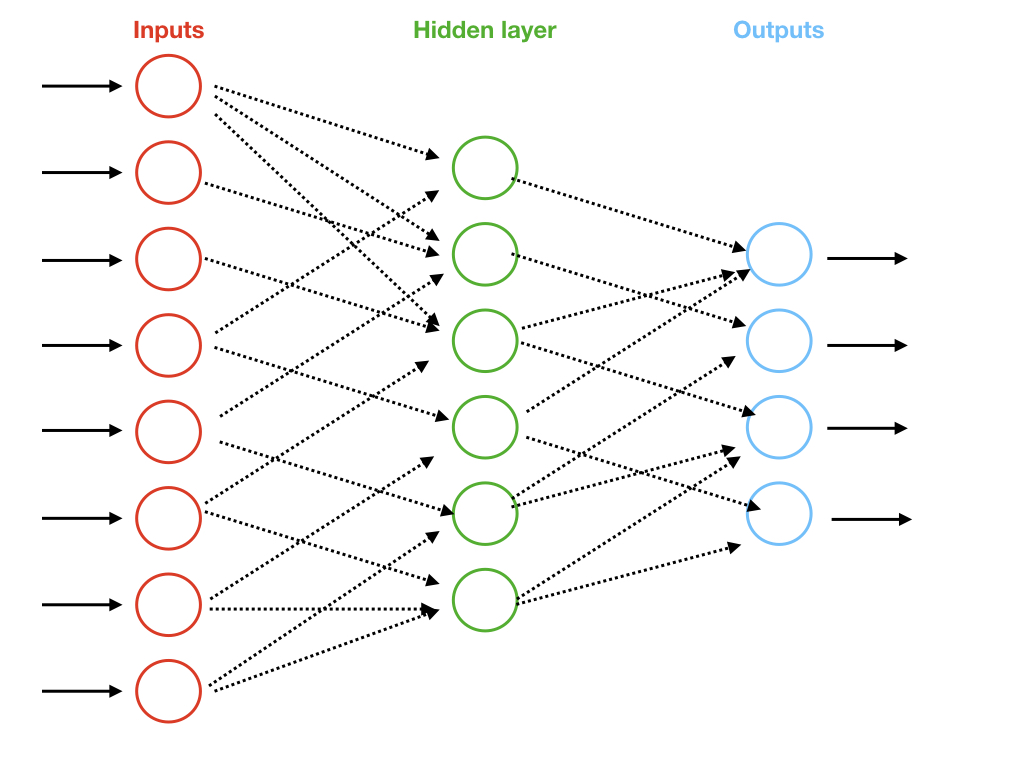
\includegraphics[scale=0.3]{exercises/ann/ann1.jpeg}
\end{figure}

\paragraph{Size of ANN}
Since the network is a fully connected with $\mathcal{R}^8\rightarrow\mathcal{R}^6\to \mathcal{R}^4$ the parameters in between layers $i$ and $j$ are estimated with:
$$|\theta_{i,j}|=(size_i+1)\times size_j$$
So for our network:
$$|\theta_{1,2}|+|\theta_{2,3}|=(8 +1) \times 6+(6 +1) \times 4=82$$
.



\paragraph{Back-Propagation}
Backpropagation algorithm is used to propagate gradient computation from the cost through the whole network. The goal is to compute the gradient of the cost function w.r.t. the parameters $\nabla_{\theta}J(\theta)$ in a simple and efficient way.

\paragraph{Backward and Forward pass}
The forward pass computes values from inputs to output and the backward pass then performs backpropagation which starts at the end and recursively applies the chain rule to compute the gradients all the way to the inputs of the circuit. The gradients can be thought of as flowing backwards through the circuit.


\paragraph{Stochastic Gradient Descend}
Stochastic Gradient Descent updates the weight parameters after evaluation of the cost function after each sample.  That is, rather than summing up the cost function results for all the sample then taking the mean, SGD updates the weights after every training sample is analyzed.

\paragraph{Back-Propagation algorithm}
\begin{itemize}
\item Requires:
	\begin{itemize}
	\item $W^i,\ i\in \braces{1,....,l}$: weight matrices
	\item $b^i,\ i\in \braces{1,....,l}$: bias matrices
	\item $x$: input value
	\item $t$: target value
	\end{itemize}
\item Forward step

\begin{itemize}
\item $h^0=x$
\item \textit{for\ k\ in\ range(1,l):}
\item $a^k=b^k+W^kh^{k-1}$
\item $h^k=f(\alpha^k)$
\item \textit{end for}
\end{itemize}

\item Backward step

\begin{itemize}
	\item $g \leftarrow \nabla_YJ=\nabla_yL(t,y)$
	\item \textit{for k=l,l-1,...1 do}
	\item $g \leftarrow \nabla_{\alpha^k}J=g \odot f' (\alpha^k)$: propagate gradient to pre-non linearity activations
	\item $\nabla_{b^k}J=g$
	\item $\nabla_{W^k}J=g(h^{k-1})^T$
	\item $g \leftarrow \nabla_{h^{k-1}}J=(W^k)^Tg$ propagate gradients to the next lower level hidden layer
	\item \textit{end for loop}
\end{itemize}

\end{itemize}


\subsection{Deep FNN}

\begin{figure}[H]
    \centering
    \includegraphics[scale=0.5]{exercises/ann/ex2.png}
\end{figure}


\paragraph{Formalization}
It is trivial to see that we need to FNN to perform a regression.
Our output will have the form:
$$y=w_{out}^T\times h+b$$
Where:
\begin{itemize}
\item $w_{out}$: are the weights associated with the output
\item $h$ is the last hidden layer's output. It can also be seen as a concatenation of multiple functions.
\item $b$ is the bias term
\end{itemize}
Since the requirements are for the FNN to be deep, but no depth is specified, we can use one hidden layer of the kind:
$$h=\phi(x^TW+c_i)$$
Where:
\begin{itemize}
\item $\phi$ is a non linearity of some kind (called activation function). We can take it to be $\phi(a)=\max(0,a)$
\item $W$ is the weight matrix associated with the hidden unit(s).
\item $c_i$ is another bias term 
\end{itemize}

So the final form for the model would be:
$$y(x)=w_{out}^T\times \phi(x^TW+c_i)+b$$

\paragraph{Activation functions}
Since this is a regression problem the activation function will be the Identity function which is simply:
$$y=W^Th+b$$
For the hidden units we can use ReLu:
$$g(\alpha)=max(0,\alpha)$$

\paragraph{Cost function }
The cost function will be the ML:
$$J(\theta)=-ln(P(t|x,\theta))$$

\subsection{BackProp, SGD}

\begin{figure}[H]
    \centering
    \includegraphics[scale=0.5]{exercises/ann/ex3.png}
\end{figure}

\paragraph{BackProp}
The backpropagation is used to compute the gradient from the cost to the whole network. That is, when the network has  classified some input $x$ as $y\neq t$, the gradient is computed.

\paragraph{Forward and backward pass}
The backprop algorithm first execute a forward pass in which the hidden units estimate their output bu multiplying input per weight. Then the gradient of the error is computed and passed backward to adjust the weights.

\paragraph{SGD}
The SGD is a training algo which uses backprop: it takes a sample of elements, compute the gradient estimates and updates the parameters.

\paragraph{Steps of backprop}
The forward steps all weights are unchanged:
\begin{enumerate}
\item for every layer multiply input per weight
\item pass the result into the activation function
\item at the end, the outputs units use the weights from the hidden units to compute the output
\item the output passes into the activation function
\end{enumerate}
Once the output is computed, the error can be estimated.\\
The backprop :
\begin{enumerate}
\item for each output unit, multiply the error's gradient into the precedent hidden unit
\item update the weights accordingly
\end{enumerate}

\subsection{Dimension}

\begin{figure}[H]
    \centering
    \includegraphics[scale=0.5]{exercises/ann/ex4.png}
\end{figure}

\paragraph{Dimension}
Since we are not caring about the number of parameters, but rather about the dimension of $W$ (the difference is the lack of a bias term), we can use the formula:
$$W=Y_i\times X_{i+1}$$
Which states that the dimension is equal to the product of:
\begin{itemize}
\item dimension  of the output $Y_i$ of the previous layer $i$
\item with the dimension of the input  $X_{i+1} $ of the next layer
\end{itemize}  
With this we get:
$$W_1=128*50 =6400$$
While the output layer has:
$$W_2=50*10 =500$$

\paragraph{Formula}
The output of the hidden neurons are given by:
$$a_i=f(x*w_i)$$
Where $f$ is the activation function.\\
The final outputs is computed as follows:
$$y=\sum_i f_{out}(a_i)$$

\subsection{Perceptron}

\begin{figure}[H]
    \centering
    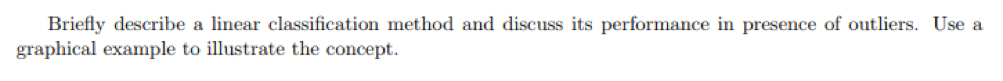
\includegraphics[scale=0.6]{exercises/ann/ex5.png}
\end{figure}

\paragraph{Classification}
Given a set of inputs $X=x_1,x_2,\dots, x_n$ and a set of weights $W=w_1,w_2,\dots,w_n$ the perceptron classifies an input with:
$$\sigma(W\cdot X)$$
where the function $\sigma$ is 1 if $W\cdot X >0$ and 0 elsewhere.

\paragraph{Training}
The training comes by updating the weights as follows:
$$w_i=w_i+\eta \sum_n (t_n-w^tx)x_{i,n}$$
Where:
\begin{itemize}
\item $\eta$ is the learning rate
\item $t_n$ is the true class of sample $x_n$
\end{itemize}

\paragraph{Convergence}
The perception training can converge only if the data is linearly separable and $\eta$ is sufficiently small.


\section{SVM}


\subsection{Slack variables}

\begin{figure}[H]
    \centering
    \includegraphics[scale=0.5]{exercises/svm/ex1.png}
\end{figure}

\paragraph{Plot}
\begin{figure}[H]
    \centering
    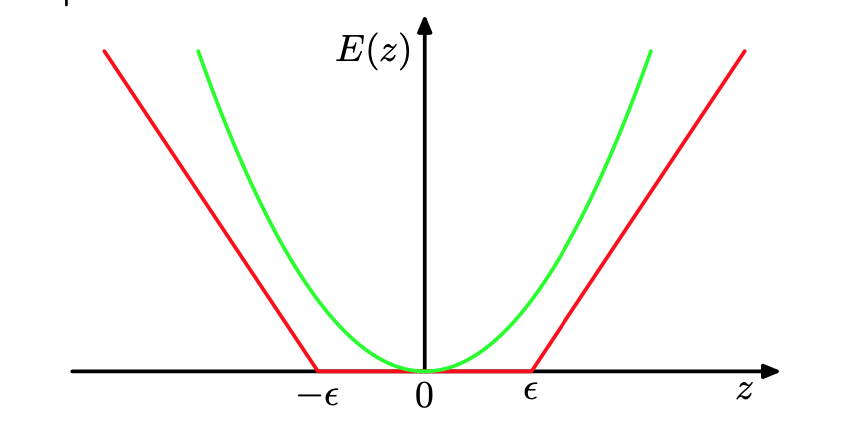
\includegraphics[scale=0.6]{exercises/svm/ex1_sol1.png}
\end{figure}
The insensitive error function is reported in the above figure.\\
The difficulty comes from the non differenciability of the $E$ (red) function.

\paragraph{Slack Variables}
The slack variables are introduced to relax the constraint from hard (no points closer than $\eta$ to the splitting plane) to soft (some points are allowed).


\subsection{Maximal Margins}

\begin{figure}[H]
    \centering
    \includegraphics[scale=0.5]{exercises/svm/ex2.png}
\end{figure}

\paragraph{Description}
Having a dataset of two linearly separable classes, we can use a line to split the space into two parts.\\
Rather than a line we have a family of lines constrain into a small space.\\
The question is which line is the best one?\\
Maximize margins between the line and the support vector to find the optimal one.

\begin{figure}[H]
    \centering
    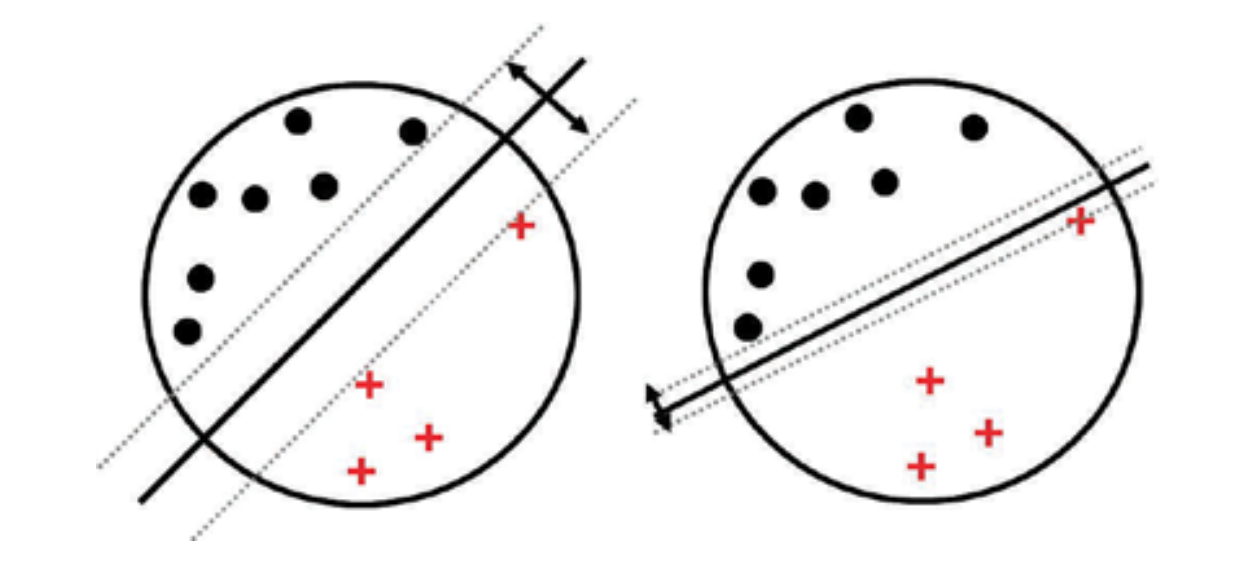
\includegraphics[scale=0.6]{exercises/svm/ex2_sol1.png}
\end{figure}

\paragraph{Maximum margin for classification}
Optimization problem for determining w (dimension $|X|$) transformed in an optimization problem for determining a (dimension $|D|$).\\
Efficient when $|X| < |D|$ (most of ai will be zero). Very useful when $|X|$ is large or infinite.


\subsection{SVM vs Perceptron}

\begin{figure}[H]
    \centering
    \includegraphics[scale=0.5]{exercises/svm/ex3.png}
\end{figure}

\paragraph{Plot}
\begin{figure}[H]
    \centering
    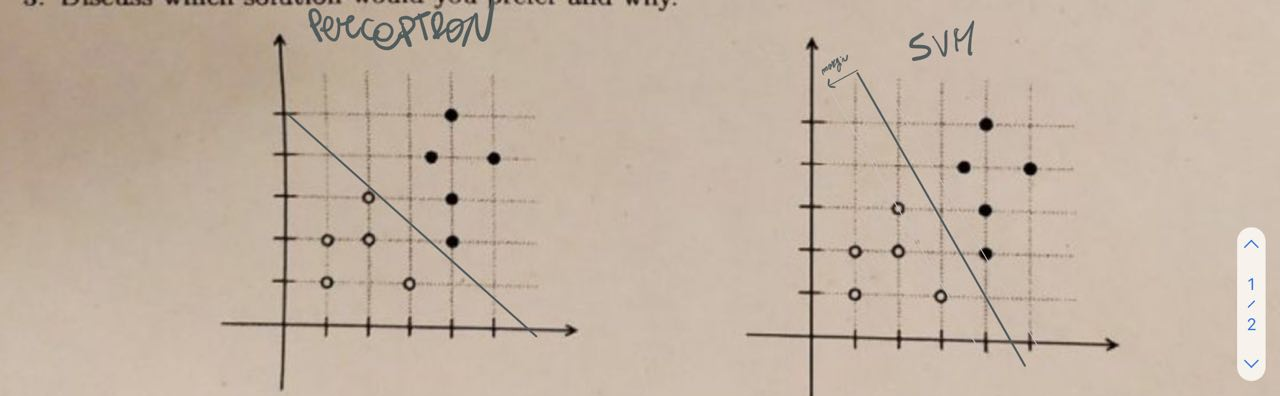
\includegraphics[scale=0.3]{exercises/svm/ex3_sol1.jpg}
\end{figure}

\paragraph{Describe}
svm is better because it finds the best hyperlplane that maximize the the distances between two classes, so it provides a better accuracy, and it takes care about just a few points( points closer to the margin). \\

The svm works even for non linearly separable dataset, using kernel trick. perceptron, instead, finds a lines that divides two classes, but its not optimal.


\section{CNN}


\subsection{Dimensions}
\begin{figure}[H]
    \centering
    \includegraphics[scale=0.5]{exercises/cnn/ex1.png}
\end{figure}

\paragraph{Dimensions}
Given:
\begin{itemize}
\item $s$ the stride 
\item $p$ the padding
\item $w_i$: the output width (first dimension)
\item $h_i$: the output height (second dimension)
\item $d_i$: the output color (third dimension)
\item $w_i\times h_i\times d_i$: output dimension of layer i
\item $n_i\times m_i$: the dimension of the kernel for conv $i$
\item $\theta$: total number of parameters
\item $y_i$: output feature map of layer i.
\item $x_i$: input feature map of layer i.
\end{itemize}

We have that the following hold for a CNN layer:
\begin{equation}
\begin{aligned}
w_i=\frac{w_{i-1}-n+2p}{s}+1\\
h_i=\frac{h_{i-1}-m+2p}{s}+1\\
d=y_i\\
\theta_i=(n_i\cdot m_i \cdot x_i+1)\cdot  y_i 
\end{aligned}
\end{equation}

For a fully connected layer:
$$\theta_i=(x_i +1)\cdot y_i $$

So, using the above equation we have:
\begin{itemize}
\item Input $1242 \times 378 \times 3$
\item conv1 : 
\begin{equation}
\begin{aligned}
w_{c1}=\frac{1242 -5+2\cdot 2}{1}+1=1242\\
h_{c1}=\frac{378-5 +2\cdot 2}{1}+1=378\\
d_{c1}=64\\
\theta_{c1}=(5\cdot 5\cdot 3+1)\cdot 64=4864
\end{aligned}
\end{equation}
\item relu1: no change
\item pool1 : 
\begin{equation}
\begin{aligned}
w_{p1}=\frac{1242 -2+2\cdot 0}{2}+1=621\\
h_{p1}=\frac{378-2 +2\cdot 0}{2}+1=189\\
d_{p1}=64\\
\end{aligned}
\end{equation}
\item conv2 : 
\begin{equation}
\begin{aligned}
w_{c2}=\frac{621 -3+2\cdot 0}{2}+1=310\\
h_{c2}=\frac{189-3 +2\cdot 0}{2}+1=94\\
d_{c2}=128\\
\theta_{c2}=(3\cdot 3\cdot 64+1)\cdot 128=73856
\end{aligned}
\end{equation}
\item relu2: no change
\item pool2 : 
\begin{equation}
\begin{aligned}
w_{p2}=\frac{310 -2+2\cdot 0}{4}+1=78\\
h_{p2}=\frac{94-2 +2\cdot 0}{4}+1=24\\
d_{p2}=128\\
\end{aligned}
\end{equation}
\end{itemize}

So the output is of dimensions $78\times 24\times 128$ and the total number of weights is:
$$\theta=\theta_{c1}+\theta_{c2}=78720$$


\subsection{Overfitting}
\begin{figure}[H]
    \centering
    \includegraphics[scale=0.5]{exercises/cnn/ex2.png}
\end{figure}

The usual approach can be taken to prevent overfitting:
\begin{itemize}
\item Data augmentation: especially for image, you can rotate them, introduce noise or change colors
\item Dropout: drop neuron who's connection are not often used
\item L1/L2 regularization.
\end{itemize}

\section{PCA}

\subsection{Exercise}

\begin{figure}[H]
    \centering
    \includegraphics[scale=0.7]{exercises/other/ex1.png}
\end{figure}

\paragraph{Formula}
The points  $x$ can be expressed in the basis of the PC $\hat{x}$ with a simple projection on the direction $u_i$:
$$\hat{x}_n=\sum_i(x^T_nu_i)u_i$$

\paragraph{Data description}
Yes because even if in theory there are as many dimension as there are pixels in the image (assuming black/white), in practice you can fully recover every image using 3 dimensions: x, y of the center and an angle of rotation because images are all the same, so you need no extra info about the image itself, only about its position

\subsection{Explanation,Algo }

\begin{figure}[H]
    \centering
    \includegraphics[scale=0.5]{exercises/pca/ex2.png}
\end{figure}

\paragraph{Dimension}
The data dimensionality is $D=144$, since this is the total number of pixels.. On the other hand, the intrinsic dimensionality is just $D=3$ two for the coordinates and one for the angle rotation.

\paragraph{Data projection}
Since we already have the principal components we can just apply the projection formula:
$$\hat{x}_n=\sum_i(x^T_nu_i)u_i$$

\paragraph{Explanation}
M should be at least equal to the number of intrinsic dimension but could also increase if there is a high enough gain in accuracy.



\section{Other}


\subsection{Boosting}

\begin{figure}[H]
    \centering
    \includegraphics[scale=0.8]{exercises/other/ex1.png}
\end{figure}

\paragraph{Boosting}
In supervised learning, boosting converts weak learners to strong ones. A weak learner is defined to be a classifier that is only slightly correlated with the true classification (it can label examples better than random guessing). In contrast, a strong learner is a classifier that is arbitrarily well-correlated with the true classification.

\paragraph{AdaBoost}
No prior knowledge about base learner is required, no parameters to tune (except for M), can be combined with any method to find base learners and theoretical guarantees given enough data and base learners with moderate accuracy.\\
The error function to minimize is:
\[J_m=\sum_{n=1}^N w_n^{(m)}\mathcal{I}(y_m(x_n)\neq t_n)\]
Given 
\begin{itemize}
\item $\epsilon_m = \frac{\sum_{n=1}^N w_n^{(m)}\mathcal{I}(y_m(x_n)\neq t_n}{\sum_{n=1}^N w_n^{(m)}}$
\item $\alpha=ln(\frac{1-\epsilon_m}{\epsilon_m})$
\end{itemize}
The output of the linear classifier is:
\[Y_m(x)=sign(\sum_{m=1}^M\alpha_my_m(x))\]




\subsection{Unsupervised}

\begin{figure}[H]
    \centering
    \includegraphics[scale=0.5]{exercises/other/ex3.png}
\end{figure}


\paragraph{Definition}
Unsupervised learning refers to the use of artificial intelligence (AI) algorithms to identify patterns in data sets containing data points that are neither classified nor labeled.

\paragraph{Example}
Clustering of similar people based on movies they watched.

\paragraph{Solution}
The clustering based on k-means could cluster together people who like more horrors or action movies.


\subsection{Gram, Kernel}

\begin{figure}[H]
    \centering
    \includegraphics[scale=0.5]{exercises/other/ex4.png}
\end{figure}
\paragraph{Gram Matrix}
Given some kernel $k(x_i,x_j)$, the Gram Matrix $K=\bm{XX^T}$ is a $N\times N$ symmetric matrix of the form:
\[K_{nm}=k(x_n,x_m)\]

\paragraph{Kernalized regression}
Considering a linear kernel $k(x,x')=x^Tx'$ we can rewrite the model as:
\[y(x)=\sum_{i=1}^N\alpha_i k(x_i,x)\]
having:
\[\alpha=(K+\lambda I)^{-1}t\]


\subsection{AutoEncoder}
Describe what is the architecture of an autoencoder and its purpose.

\paragraph{Description}
The architecture of an autoencoder is similar to the one of a cnn, but flipped. That is it takes as input a random vector and returns an image.\\
It is usually trained in an adversarial fashion to keep the supervision cycle closed.\\
It's purpose is to encode a sparse representation (e.g. words) into a small vector (dimensionallity reduction)

\subsection{Multiple Learners}

\begin{figure}[H]
    \centering
    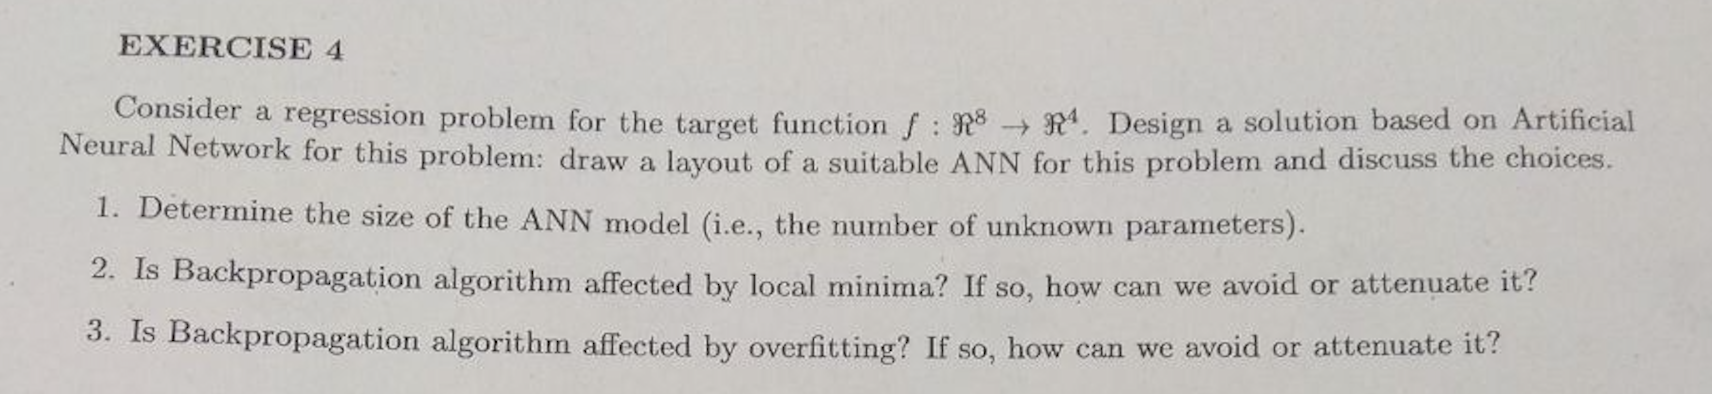
\includegraphics[scale=0.5]{exercises/other/ex6.png}
\end{figure}

\paragraph{Method}
A method to achieve such results we can use the voting method in which we train each classifier in parallel on the trainset. For the prediction we take the most predicted class (for classification) or the sum of the predictions (for regression).

\paragraph{Proprieties}
A base propriety for each classifier is that they have to achieve a sufficient accuracy on their own. Implementing multi learners methods where the indiviual classifiers do not achieve a more than $10\%$ accuracy is not advised.

\subsection{Gaussian Mixture models GMM}

\begin{figure}[H]
    \centering
    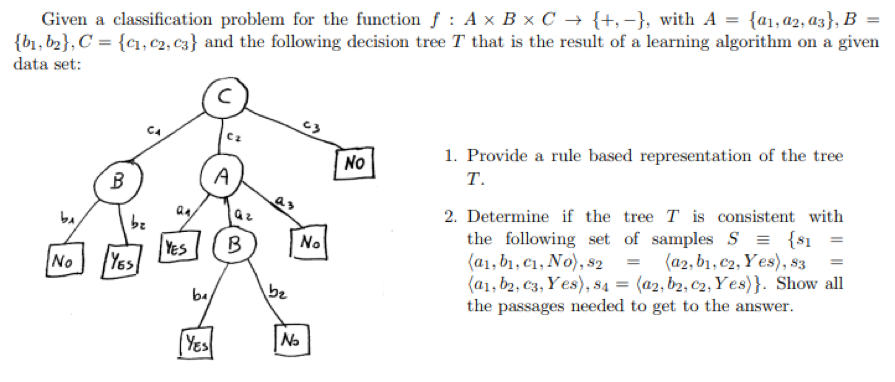
\includegraphics[scale=0.7]{exercises/other/ex7.png}
\end{figure}

\paragraph{Definition}
A gaussian mixture model has the form:
$$p(x)=\prod_k \pi_k N(x,\mu_k,\Sigma_k)$$
The parameters are given by $\mu_k, \Sigma_k, \pi_k$

\paragraph{Model size }
Since $K=3$ the parameters are: 
\begin{itemize}
\item 3 means $\mu_1,\mu_2,\mu_3$ 
\item 3 mixture intensities $\pi_1,\pi_2,\pi_3$ 
\item 3 covariance matrices $\Sigma_1,\Sigma_2,\Sigma_3$. Notice that these matrices are $3\times 3$ each, so, in terms of parameters, they count as $36$ elements.
\end{itemize}
The total size of the model is $9$.

\subsection{Generative vs Discriminative Probabilistic}

\begin{figure}[H]
    \centering
    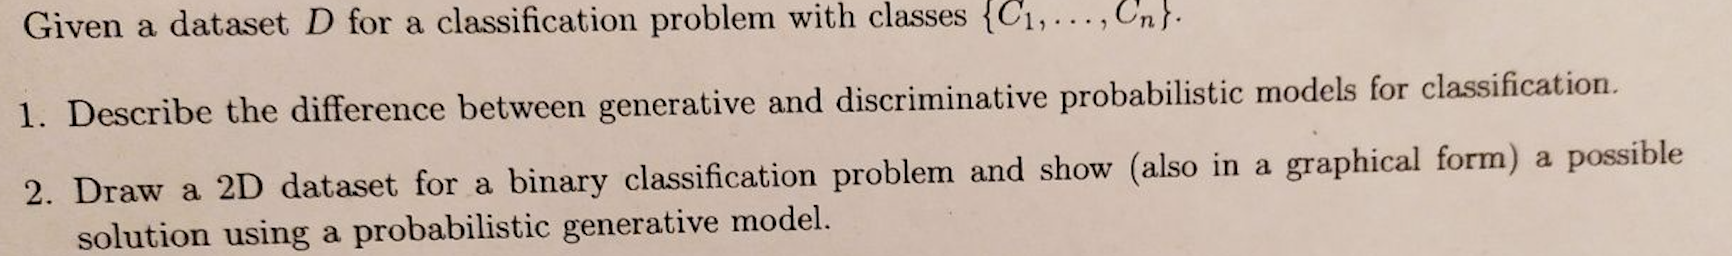
\includegraphics[scale=0.5]{exercises/other/ex8.png}
\end{figure}

\paragraph{Difference}
the difference is that the generative model estimates $P(C_i|x)$ with the bayes theorem while the discriminative uses the model directly.

